In the table below, place the numbers $1-12$ in the shaded cells. You start at the center cell (marked with $*$ ). You repeatedly move up, down, left, or right, chosen uniformly at random each time, until reaching a shaded cell. Your score is the number in the shaded cell that you end up at.

Let $m$ be the least possible expected value of your score (based on how you placed the numbers), and $M$ be the greatest possible expected value of your score. Compute $m \cdot M$.

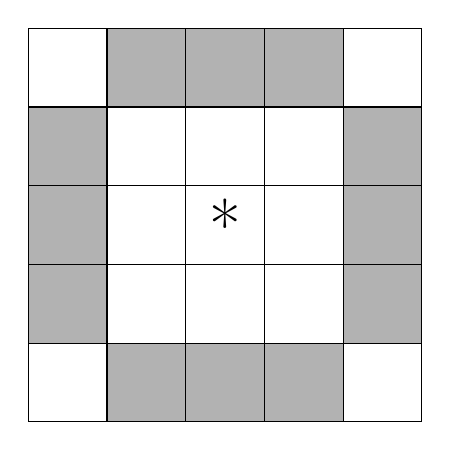
\begin{tikzpicture}
    \def\grayfill{black!30}
    
    \foreach \x in {0,1,2,3,4} {
        \foreach \y in {0,1,2,3,4} {
            \ifthenelse{\x=0 \AND \y=0}{}
            {\ifthenelse{\x=0 \AND \y=4}{}
            {\ifthenelse{\x=4 \AND \y=0}{}
            {\ifthenelse{\x=4 \AND \y=4}{}
            {\filldraw[white, draw=black] (\x,\y) rectangle ++(1,1);}
            }}}}
        }
    
    \foreach \p in {(0,1), (0,2), (0,3), (1,0), (2,0), (3,0), (4,1), (4,2), (4,3), (1,4), (2,4), (3,4)} {
        \filldraw[\grayfill, draw=black] \p rectangle ++(1,1);
    }

    \node at (2.5,2.5) {\Huge *};

\end{tikzpicture}